\documentclass[11pt]{beamer}
\usepackage[utf8]{inputenc}
\usepackage[T1]{fontenc}
\usepackage{lmodern}
\usepackage{graphicx}
\usepackage{amsmath}
\usepackage[english]{babel}
\usetheme{AnnArbor}
\date{}
\begin{document}
	\author{A R Bathri Narayanan; Carin Samer}
	\title{Theoretical studies of Ej/Ec ratio and applying it to solve a theoretical physics problem}
	%\subtitle{}
	%\logo{}
	\institute{UM DAE CEBS, India; Alexandria, Egypt}
	%\date{}
	%\subject{}
	%\setbeamercovered{transparent}
	%\setbeamertemplate{navigation symbols}{}
	\begin{frame}[plain]
		\maketitle
	\end{frame}
	
		\begin{frame}
		\frametitle{How can you modify Superconducting Qubits (Josephson Junctions and dc-SQUIDs)}
		Josephson Junctions are represented by 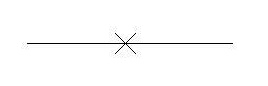
\includegraphics[width=1 cm]{sc7.png}. This has the properties
		\[V_J=\frac{\Phi_0}{2\pi}\frac{d\varphi_J}{dt}\]
		\[I_J=I_c sin \varphi_J\]
		\[L_J=\frac{\phi_J}{I_csin(2\pi\phi_J/\phi_0)}=\frac{\phi_0\varphi_J}{2\pi I_c sin\varphi_J}\]
		The circuit can be drawn like\\
		\begin{center}
			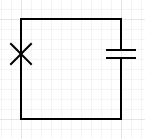
\includegraphics[width=2cm]{sc8.png}
		\end{center}
			\end{frame}
		
		\begin{frame}
			\frametitle{Analog gravity using superconducting qubits}
			We construct an infinite circuit like
			\begin{center}
				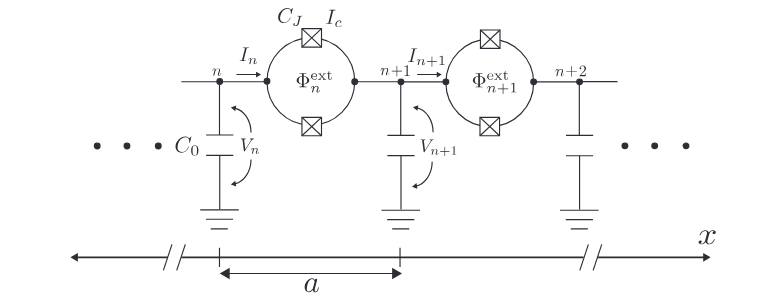
\includegraphics[width=8 cm]{sc9.png}
			\end{center}
			Now, we apply Kirchoff law and Faraday's law as
			\[I_n - I_{n+1}=\frac{dQ_{n+1}}{dt}\]
			\[V_n-V_{n+1}=\frac{\Phi_0}{2\pi}\frac{d\varphi_{Jn}}{dt}\]
		\end{frame}
		
		\begin{frame}
			\frametitle{Obtaining the equation of motion}
			Plugging in the formulas obtained for Josephson junctions, we can obtain the current entering the nth unit cell as
			\[I_n=2 C_J \frac{\Phi_0}{2\pi}\frac{d^2\varphi_{Jn}}{dt^2}+2I_ccos\bigg(\frac{\pi \Phi^{ext}_n}{\Phi_0}\bigg)sin\varphi_{Jn}\]
			Applying $\varphi_{Jn}$=$\varphi_{n}$-$\varphi_{n+1}$ and plugging the above in the $V_n$ equation, we obtain
			\[(C_0+4C_J)\bigg(\frac{\Phi_0}{2\pi}\bigg)^2\frac{d^2\varphi_{n}}{dt^2}-2C_J\bigg(\frac{\Phi_0}{2\pi}\bigg)^2\bigg( \frac{d^2\varphi_{n-1}}{dt^2}+\frac{d^2\varphi_{n+1}}{dt^2}  \bigg)\]
			\[=-2E_Jcos\bigg(\frac{\pi \Phi^{ext}_n}{\Phi_0}\bigg)sin(\varphi_{n}-\varphi_{n+1})+2E_Jcos\bigg(\frac{\pi \Phi^{ext}_{n-1}}{\Phi_0}\bigg)sin(\varphi_{n-1}-\varphi_{n})\]
		\end{frame}
		
		\begin{frame}
			\frametitle{Obtaining the EM phase speed}
			We can guess the Lagrangian, and eventually the Hamiltonian, which is nothing but
			\[H=\int_{-\infty}^{\infty}dx\bigg[\bigg(\frac{2\pi}{\Phi_0}\bigg)^2\frac{p^2}{2\mathcal{C}}+E_Jacos\bigg(\frac{\pi \Phi^{ext}}{\Phi_0}\bigg)\bigg(\frac{\partial\varphi}{\partial x}\bigg)^2\bigg]\]
			Of course we make a few approximations like the continuum approximation, neglecting the Josephson junction capacitance term. 
			We get the following wave equation
			\[\frac{\partial^2\varphi}{\partial t^2}=\frac{\partial}{\partial x}\bigg(c^2\frac{\partial \varphi}{\partial x}\bigg),c=\frac{1}{\sqrt{\mathcal{L}\mathcal{C}}}\]
			Where,
			\[\mathcal{C}=C_0/a,\mathcal{L}=\frac{\Phi_0}{4\pi I_ca}sec\bigg(\frac{\pi \Phi^{ext}}{\Phi_0}\bigg)\]
		\end{frame}
		
			\begin{frame}
			\frametitle{Getting the covariant wave equation}
			Now, we transform as x'=x-ut, t'=t, the wave equation becomes 
			\[\bigg(-\frac{\partial^2}{\partial t^2}+2u\frac{\partial^2}{\partial x\partial t}+\frac{\partial}{\partial x}\big(c^2-u^2\big)\frac{\partial}{\partial x}\bigg)\varphi=0=\frac{1}{\sqrt{-g}}\partial_\mu(\sqrt{-g}g^{\mu\nu}\partial_\nu\varphi)\]
			Where,
			\[ g^{\mu\nu}=\frac{1}{c}
			\begin{pmatrix}
				-1 & u \\
				u & c^2-u^2 
			\end{pmatrix}
			\]
			We finally take the Hawking temperature
			\[T_H=\frac{\hbar}{2\pi k_B}\bigg|\frac{\partial c}{\partial x}\bigg|_{x_h}\]
			And plug in the respective values to get an estimate (for $\bigg|\frac{\partial c}{\partial x}\bigg|_{x_h}$$\approx$0.01$c_0$/a, $C_0$=1$\mu$ F, $I_c$=5$\mu$A, $T_h$= 70 mK)
		\end{frame}
		
		\begin{frame}{The Ej/Ec ratio}
			Usually in transmon qubits, the Ej, that is Josephson energy of the circuit, is greater than Ec, the capacitive energy of the circuit. To put it mathematically, Ej/Ec >>1.\\
			 This gives an advantage of  less interference of charge noise, and a disadvantage of anharmonicity. But this can be overcome by tuning the microwave pulse appropriately.\\
			 We try varying the Ej/Ec ration of a single tunable transmon qubit, which forms a basic building block of our system.
	\end{frame}
	
\begin{frame}{The Ej/Ec ratio}
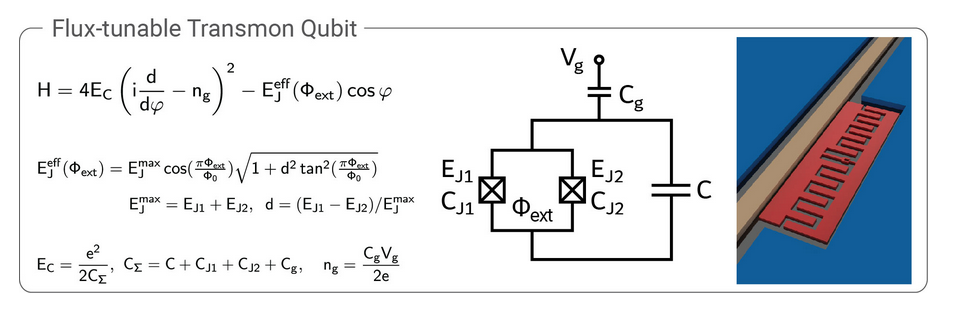
\includegraphics[width=8 cm]{sc10.png} Taken from scqubits
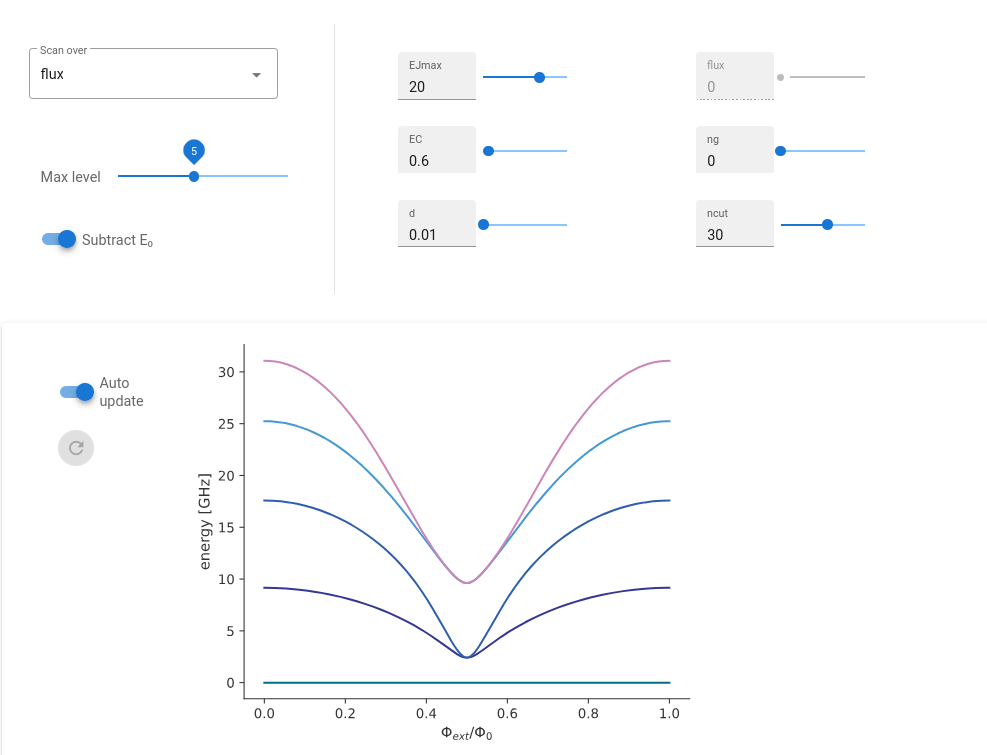
\includegraphics[width=3.7 cm]{sc11.png}
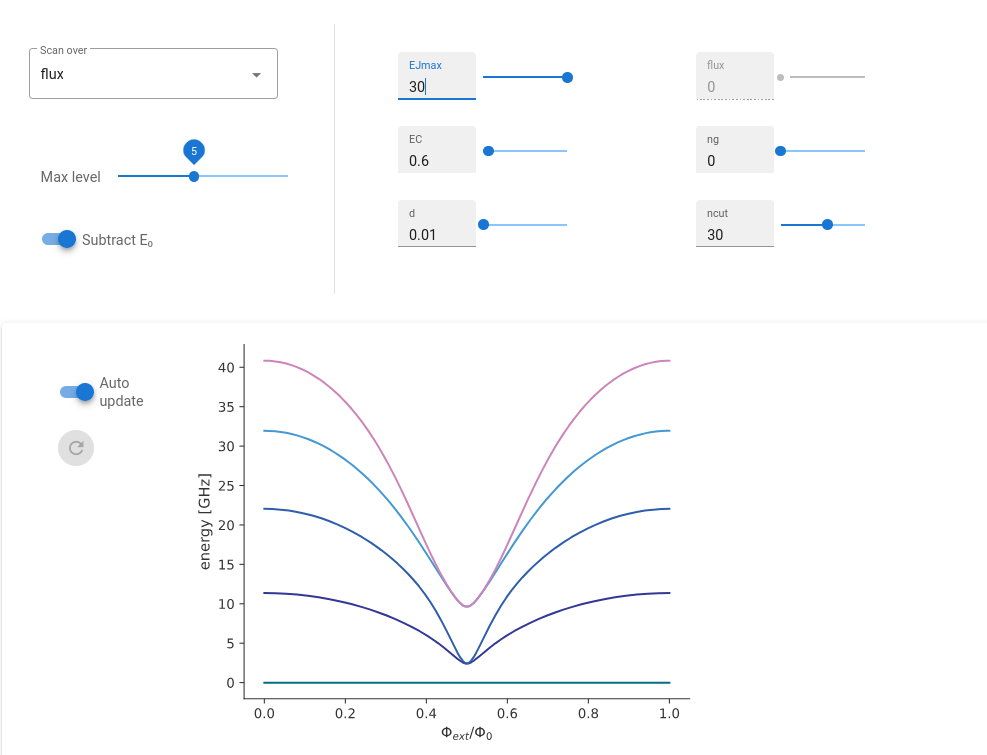
\includegraphics[width=3.7 cm]{sc12.png}
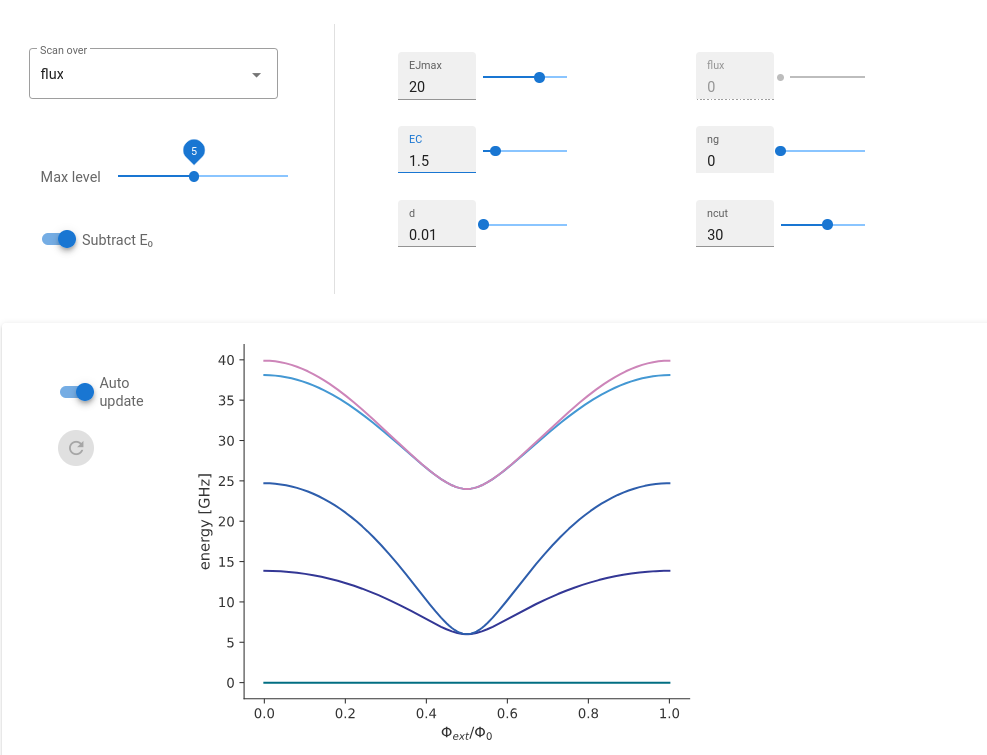
\includegraphics[width=3.7 cm]{sc13.png}
The flux graph taken for various ratios of Ej/Ec
\end{frame}

\begin{frame}{The bigger aim}
	We have constructed a circular Blencowian qubit. And we would like to analyse on this more. This resembles more like a current mirror qubit, which is even more insensitive to errors as found out by Koch.
	\begin{center}
		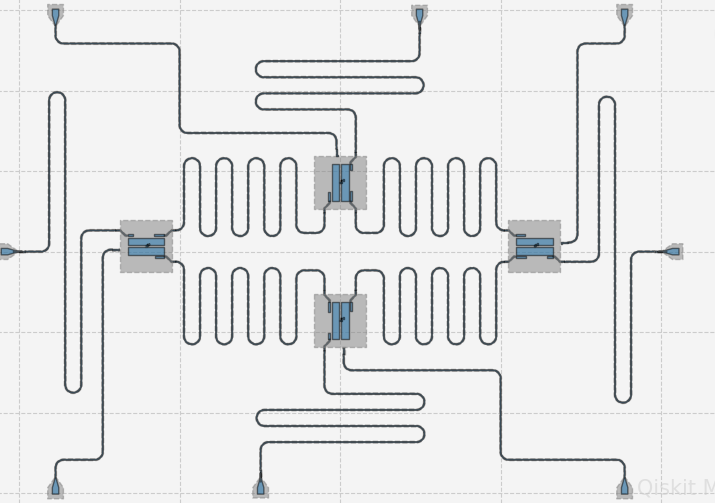
\includegraphics[width=8 cm]{sc14.png}
	\end{center}
\end{frame}

\begin{frame}{References}
	Miles Blencowe Paper on Analogue Gravity
	Sc Qubits, Qiskit Metal Documentation
\end{frame}

		
	
\end{document}